\documentclass[energies,article,submit,moreauthors]{Definitions/mdpi}
\graphicspath{{../papers/figures/}}
\setlength{\headheight}{20pt}
% Suppress the MDPI template's unassigned, metadata-derived DOI in submit mode.
\AtBeginDocument{%
  \rfoot{}%
  \fancypagestyle{plain}{\rfoot{}}%
}
\firstpage{1}
\makeatletter
\setcounter{page}{\@firstpage}
\makeatother
\pubvolume{1}
\issuenum{1}
\articlenumber{0}
\pubyear{2026}
\copyrightyear{2026}
\Title{A Viability-Shielded Adaptive ECMS for Charge-Sustaining Energy Management in a Hybrid Agricultural Tractor}
\newcommand{\orcidauthorA}{0009-0005-1928-6218}
\Author{Chenyu Cui$^{1}$, Peng Wang$^{1}$ and Yucheng Zhang$^{1,}$*\orcidA{}}
\AuthorNames{Chenyu Cui, Peng Wang and Yucheng Zhang}
\address{%
$^{1}$ \quad Prospective Research Laboratory, Institute of Computing Technology, Chinese Academy of Sciences, Beijing 100190, China}
\corres{Correspondence: zhangyucheng@ict.ac.cn}
\datereceived{}
\daterevised{}
\dateaccepted{}
\datepublished{}
\abstract{Charge-sustaining energy management for hybrid agricultural tractors must separate economic decisions from hard power and terminal-energy feasibility. This study develops a viability-shielded adaptive equivalent-consumption minimization (ECMS) controller in a parameterized OS-ECVT virtual prototype. The controller uses a public task-phase SOC corridor, finite engine-speed and power actions, a causal electric-reserve rule, minimum engine on/off dwell, and an internal viability shield covering the engine ramp, MG1/MG2 limits, battery internal resistance, SOC bounds, and terminal SOC closure. No terminal SOC command is appended by the experiment runner. On 20 frozen stochastic agricultural cycles, the proposed controller was strictly valid on 20/20 paths and achieved a 5.68\% mean terminal-energy-normalized fuel reduction (95\% CI: 5.12\%--6.23\%) relative to a matched load-following baseline. A strict 0.0001 SOC audit remained valid on 20/20 paths, with a maximum absolute SOC error of 0.0000553 and a maximum observed local Python decision time of 9.50 ms. Independent deterministic, low-load, and 20-seed stochastic audits retained positive savings, whereas a declared high-variability cycle exceeded the virtual electrical envelope and was reported as infeasible. Map and battery-capacity sensitivities retained positive savings on 19/20 valid pairs; one high-demand path produced no feasible ramp-constrained action and was retained as a failure. The earlier terminal-set MPC comparison is retained as a negative control. A separate full-information oracle remains an idealized headroom diagnostic, not an online result.}
\keyword{hybrid agricultural tractor; energy management; adaptive ECMS; viability shield; terminal state of charge; model predictive control; component-map sensitivity; virtual powertrain}
\begin{document}

\section{Introduction}
Agricultural traction demand varies with soil condition, grade, vehicle speed, implement operation, and auxiliary loads. A hybrid powertrain can buffer this variation, but it can also produce misleading apparent savings when battery depletion, power shortage, or an unfavorable baseline is not controlled. The diversity of tractor hybrid architectures is illustrated by assessments of solar-assisted plug-in concepts \cite{mousazadeh2011}, parallel hybrid tractors \cite{mocera2020,mocera2020b}, and MPC-based hybrid agricultural-tractor control \cite{curiel2023}. These studies establish the relevance of power-split and supervisory decisions, while also showing why fuel figures cannot be compared without a common operating protocol.

The comparison problem is particularly acute for agricultural work cycles. Engine load and rated-power matching affect tractor fuel use \cite{jilek2008,janulevicius2010}, while steady maps omit turbocharger and other transient limits \cite{huo2018}. A reported reduction can depend on the initial and terminal state of charge (SOC), the actuator and ramp limits, the selected baseline, and whether a controller sees future demand. Thus, a virtual result should identify the information set and energy-accounting rule before it is interpreted as a controller benefit. This requirement is not unique to tractors, but it matters strongly when a controller is evaluated on a short, variable-load task.

Terminal-energy accounting is a central part of that protocol. A controller that ends a finite cycle with less battery energy than the baseline can appear to save engine fuel even when the comparison has merely shifted energy beyond the reporting window. Similarly, a low-fuel MPC trajectory is not an online result when it relies on a future load realization, an infeasible candidate set, or an unreported intervention applied after the optimizer fails. A strict comparison must therefore distinguish the policy decision, the applied engine command after limits, the terminal SOC condition, and any safety action that preserves feasibility. These distinctions make a negative or near-zero fuel result scientifically useful: they show which stated controller and map combination does not provide a benefit under the declared information set.

A second challenge is the role of component maps. The engine-efficiency map, battery resistance model, machine limits, and load construction jointly define the opportunity for power shifting in a virtual prototype. A map sensitivity can be valuable when it is reported as a mechanism test, because it reveals whether a conclusion depends on a stated low-load penalty or efficiency island. It becomes misleading only when a deliberately favourable map is presented as a calibrated tractor characteristic. The present study therefore retains both a literature-shaped map and a deliberately steep sensitivity map, applies the same hardware and terminal rules to both, and treats any contrast as conditional virtual-model evidence. This design allows the path from a declared map assumption to a reported controller outcome to be inspected directly.

This article asks two engineering questions. First, can an adaptive ECMS and an internal viability shield produce a positive, strictly charge-sustaining result without an experiment-runner terminal correction? Second, does the sign of that result persist across independent cycles, action-grid resolutions, battery capacities, and transparent engine-map changes? The purpose is not to claim a physical map for a target tractor, but to determine which conclusions survive declared changes in the theoretical virtual platform.

The study is organized around a primary V2 controller and an auditable negative-control benchmark. The V2 controller and its load-following baseline share the same power-split plant, present information, hard limits, task-phase definition, and terminal-energy rule. Development seeds are separated from holdout seeds wherever parameters are selected. The legacy MPC comparison is retained because it shows that feasibility alone does not imply a fuel benefit, while the offline oracle is kept separate from all causal statistics.

\section{Related Work}
Tractor-specific energy-management research has examined several controller families and powertrain configurations. Mocera and Som\`a analysed a parallel hybrid tractor, and Mocera subsequently reported a hardware-in-the-loop model-based design workflow \cite{mocera2020,mocera2020b}. Curiel-Olivares et al. applied MPC to a hybrid electric agricultural tractor \cite{curiel2023}. More recent work has examined deep reinforcement learning for a hybrid electric agricultural tractor \cite{wu2024} and energy management for a fuel-cell tractor hybrid system \cite{zhao2024}. These studies address valuable implementation choices, but their differing maps, cycles, reference strategies, and constraint conventions mean that their reported fuel changes are not a common causal ranking.

The broader hybrid-vehicle literature supplies the principal method families used in such comparisons. Dynamic programming offers an offline reference because it can optimize against a known trajectory \cite{xie2016}. ECMS expresses battery-energy use as an equivalent fuel cost and is attractive for real-time use \cite{musardo2005}. Stochastic and deterministic MPC formulations can incorporate predictions and constraints \cite{ripaccioli2010,zhang2017,wang2016}, but their benefit depends on the forecast information and on whether the optimization remains feasible after plant constraints are imposed. Consequently, an offline optimum or an MPC simulation with undeclared fallback should not be treated as directly comparable with a strictly causal online policy.

This work addresses that comparison gap with a viability-shielded adaptive ECMS whose terminal-energy action remains inside the controller. It also retains a shared strict protocol for map-aware ECMS, deterministic MPC, scenario MPC, and terminal-set safeguarded scenario MPC as a legacy negative-control benchmark. Every intervention is counted rather than silently treated as controller-external fallback. A full-information oracle is reported only as an explicitly idealized headroom diagnostic. The scope is deliberately limited to simulation: the component maps are defined virtual-model inputs, not claims of field, vehicle, or bench measurement.

For an energy-systems audience, the central contribution is the coupling of an economic adaptive ECMS proposal with a transparent discrete viability layer and matched terminal-energy accounting. The protocol records every safety intervention, engine start, terminal SOC residual, and invalid path. This prevents an apparently favorable fuel number from being produced by unequal residual battery energy or by an unreported post-optimization repair. The negative MPC finding remains useful as a conditional boundary and motivates the primary V2 architecture.

The contributions are as follows: (i) a causal adaptive ECMS with an internal shrinking-SOC viability shield and no runner-side terminal repair; (ii) a power-split candidate model with explicit MG1/MG2, battery, engine-ramp, start-power, minimum-dwell, and electric-reserve constraints; (iii) development/holdout separation followed by a strict $10^{-4}$ SOC audit; (iv) independent cycle, map, capacity, and action-grid audits that retain invalid paths; (v) a legacy terminal-set MPC comparison as a negative control; and (vi) an approximately 20\% full-information oracle reported only as idealized headroom. The resulting paper is a conditional theoretical energy-management study, not a claim of generic MPC superiority or measured tractor fuel economy.

\section{Materials and Methods}
\subsection{Powertrain and demand models}
The required traction power is
\begin{equation}
 P_{dem}=\frac{(F_d+F_r+mg\sin\theta)v}{\eta_t},\qquad
 F_d=K_sF_{d0}+\Delta F_d,
\end{equation}
where $K_s$ is a soil factor and $\Delta F_d$ is a stochastic disturbance. The simplified planetary relation is
\begin{equation}
 \omega_{MG1}+\kappa\omega_r=(1+\kappa)\omega_e,
\end{equation}
and the power balance is $P_{dem}=\eta_mP_e+P_{MG2}-P_{loss}$. The present implementation checks proxy MG1/MG2 speed and power boundaries but does not model a calibrated planetary gearset.

The battery uses a first-order equivalent circuit,
\begin{equation}
 V_t=V_{oc}(SOC)-I_bR(SOC,T),\qquad
 SOC_{k+1}=SOC_k-\frac{V_tI_b\Delta t}{E_b}.
\end{equation}
Battery power, SOC, engine power, motor power, regenerative power, and engine-ramp limits are imposed. The numerical maps and constraints are engineering assumptions unless explicitly described as literature-shaped.

\subsection{Control formulation}
The control architecture is shown in Figure~\ref{fig:architecture}. Four online methods are compared. Map-aware ECMS selects a present engine power from a feasible interval by minimizing \cite{musardo2005}
\begin{equation}
 J_{\mathrm{ECMS}}(P_e)=\dot m_f(P_e)+\lambda P_{b}(P_{dem}-P_e),
\end{equation}
where $\lambda$ is a fixed battery-energy equivalence factor. The nominal-phase policy uses the public recurring task phase and the present demand residual, $P_e=P_{\mathrm{phase}}+0.75(P_{dem}-P_{\mathrm{phase}})$. Its phase targets are calculated once from the zero-disturbance public task, not from any evaluated stochastic seed. Deterministic MPC evaluates a finite candidate set over an eight-sample prediction horizon. Scenario MPC evaluates the same candidates over five demand-scenario roll-outs and selects the minimum worst-scenario cost \cite{ripaccioli2010},
\begin{equation}
 \min_{u\in\mathcal{U}}\max_{\omega\in\Omega}\sum_{i=0}^{H-1}
 (w_fJ_f+w_bJ_b+w_qJ_q+w_rJ_r)+w_TJ_T.
\end{equation}
For all MPC methods, the nominal phase preview is public and the first predicted demand equals the measured current demand; no method reads an evaluated seed's future samples. This is finite-set search, not a converged QP or nonlinear-program solution. Terminal-set scenario MPC retains the same causal nominal optimizer but adds a safety filter. With $n_k$ samples remaining, its terminal-energy viability envelope is
\begin{equation}
 \mathcal{X}_k=\left[SOC_{ref}-\epsilon-\frac{P_b^{max}n_k\Delta t}{E_b},\;SOC_{ref}+\epsilon+\frac{P_b^{max}n_k\Delta t}{E_b}\right]\cap[SOC_{min},SOC_{max}],
\end{equation}
where $\epsilon=10^{-4}$. The proposed action is projected onto the current measured-load electrical/ramp set and accepted only if $SOC_{k+1}\in\mathcal{X}_{k+1}$. When the finite scenario intersection is empty, this declared internal policy replaces it and its activation is counted. This is a conditional recursive-feasibility structure, verified on the frozen virtual paths; the energy envelope is not a formal robust-feasibility proof for arbitrary unmodelled demand jumps.

The legacy finite-set comparison used the following common causal terminal-energy governor,
\begin{equation}
 P_{e,k}^{\mathrm{applied}}=\Pi_{\mathcal{F}_k}\left[P_{e,k}^{\mathrm{policy}}+
 3\frac{(SOC_0-SOC_k)E_b}{t_{\mathrm{rem},k}}\right],
\end{equation}
where $\Pi_{\mathcal{F}_k}$ denotes projection onto the instantaneous motor, battery-bus, engine-power, and applied-ramp envelope. The gain of three is identical for every legacy comparison method. This section is retained as a negative-control benchmark; it is not appended to the V2 controller.

\subsection{V2 viability-shielded adaptive ECMS}
The V2 controller removes the experiment-runner terminal correction. At each 1 s decision, the controller enumerates engine power at a frozen 5 kW grid and three engine-speed candidates. Each candidate is propagated through the same two-dimensional efficiency maps, battery OCV--resistance relation, MG1/MG2 power and speed limits, engine ramp limit, and SOC bounds used by the virtual plant. The economic score is
\begin{equation}
 J(u_k)=m_f(u_k)+\lambda_k m_{b,eq}(u_k)+w_{th}|P_{b,k}|+w_s I_{start},
\end{equation}
where $m_{b,eq}$ is the equivalent fuel associated with battery-bus energy, $w_{th}$ penalizes throughput, and $I_{start}$ penalizes an engine start. The adaptive factor is
\begin{equation}
 \lambda_k=\max\{\lambda_{min},\lambda_0+K_p(SOC^{ref}_k-SOC_k)\}.
\end{equation}
The reference $SOC^{ref}_k$ is a public four-phase task corridor that returns to $SOC_0$ during the last 120 s; it uses no evaluated-seed future demand.

The viability shield is an internal action filter. Let $\mathcal{U}_k$ be the actions satisfying the measured-demand electrical interval and applied engine-ramp constraint. A cold start can enter only the 60 kW minimum stable-power point; subsequent changes obey the 40 kW s$^{-1}$ ramp. Once started, the engine remains on for at least 5 s, and a stop lasts at least one 1 s decision sample. A current-measurement reserve rule prevents electric-only operation when its bus power would exceed 65\% of the 180 kW bus limit, leaving 35\% causal headroom for an unobserved next-step rise. The shield then retains only actions whose successor SOC lies inside a shrinking corridor $[SOC^{ref}_k-b_k,SOC^{ref}_k+b_k]$, with $b_k=b_0\rho_k^2$ and $\rho_k$ the remaining-cycle fraction. If the intersection is empty, the action minimizing successor-SOC distance is selected and the event is counted as an empty-set intervention; no external command is inserted after the controller. This is a conditional discrete-action viability construction for the declared virtual platform, not a robust proof for arbitrary unmodelled demand.

\begin{figure}[H]
\centering
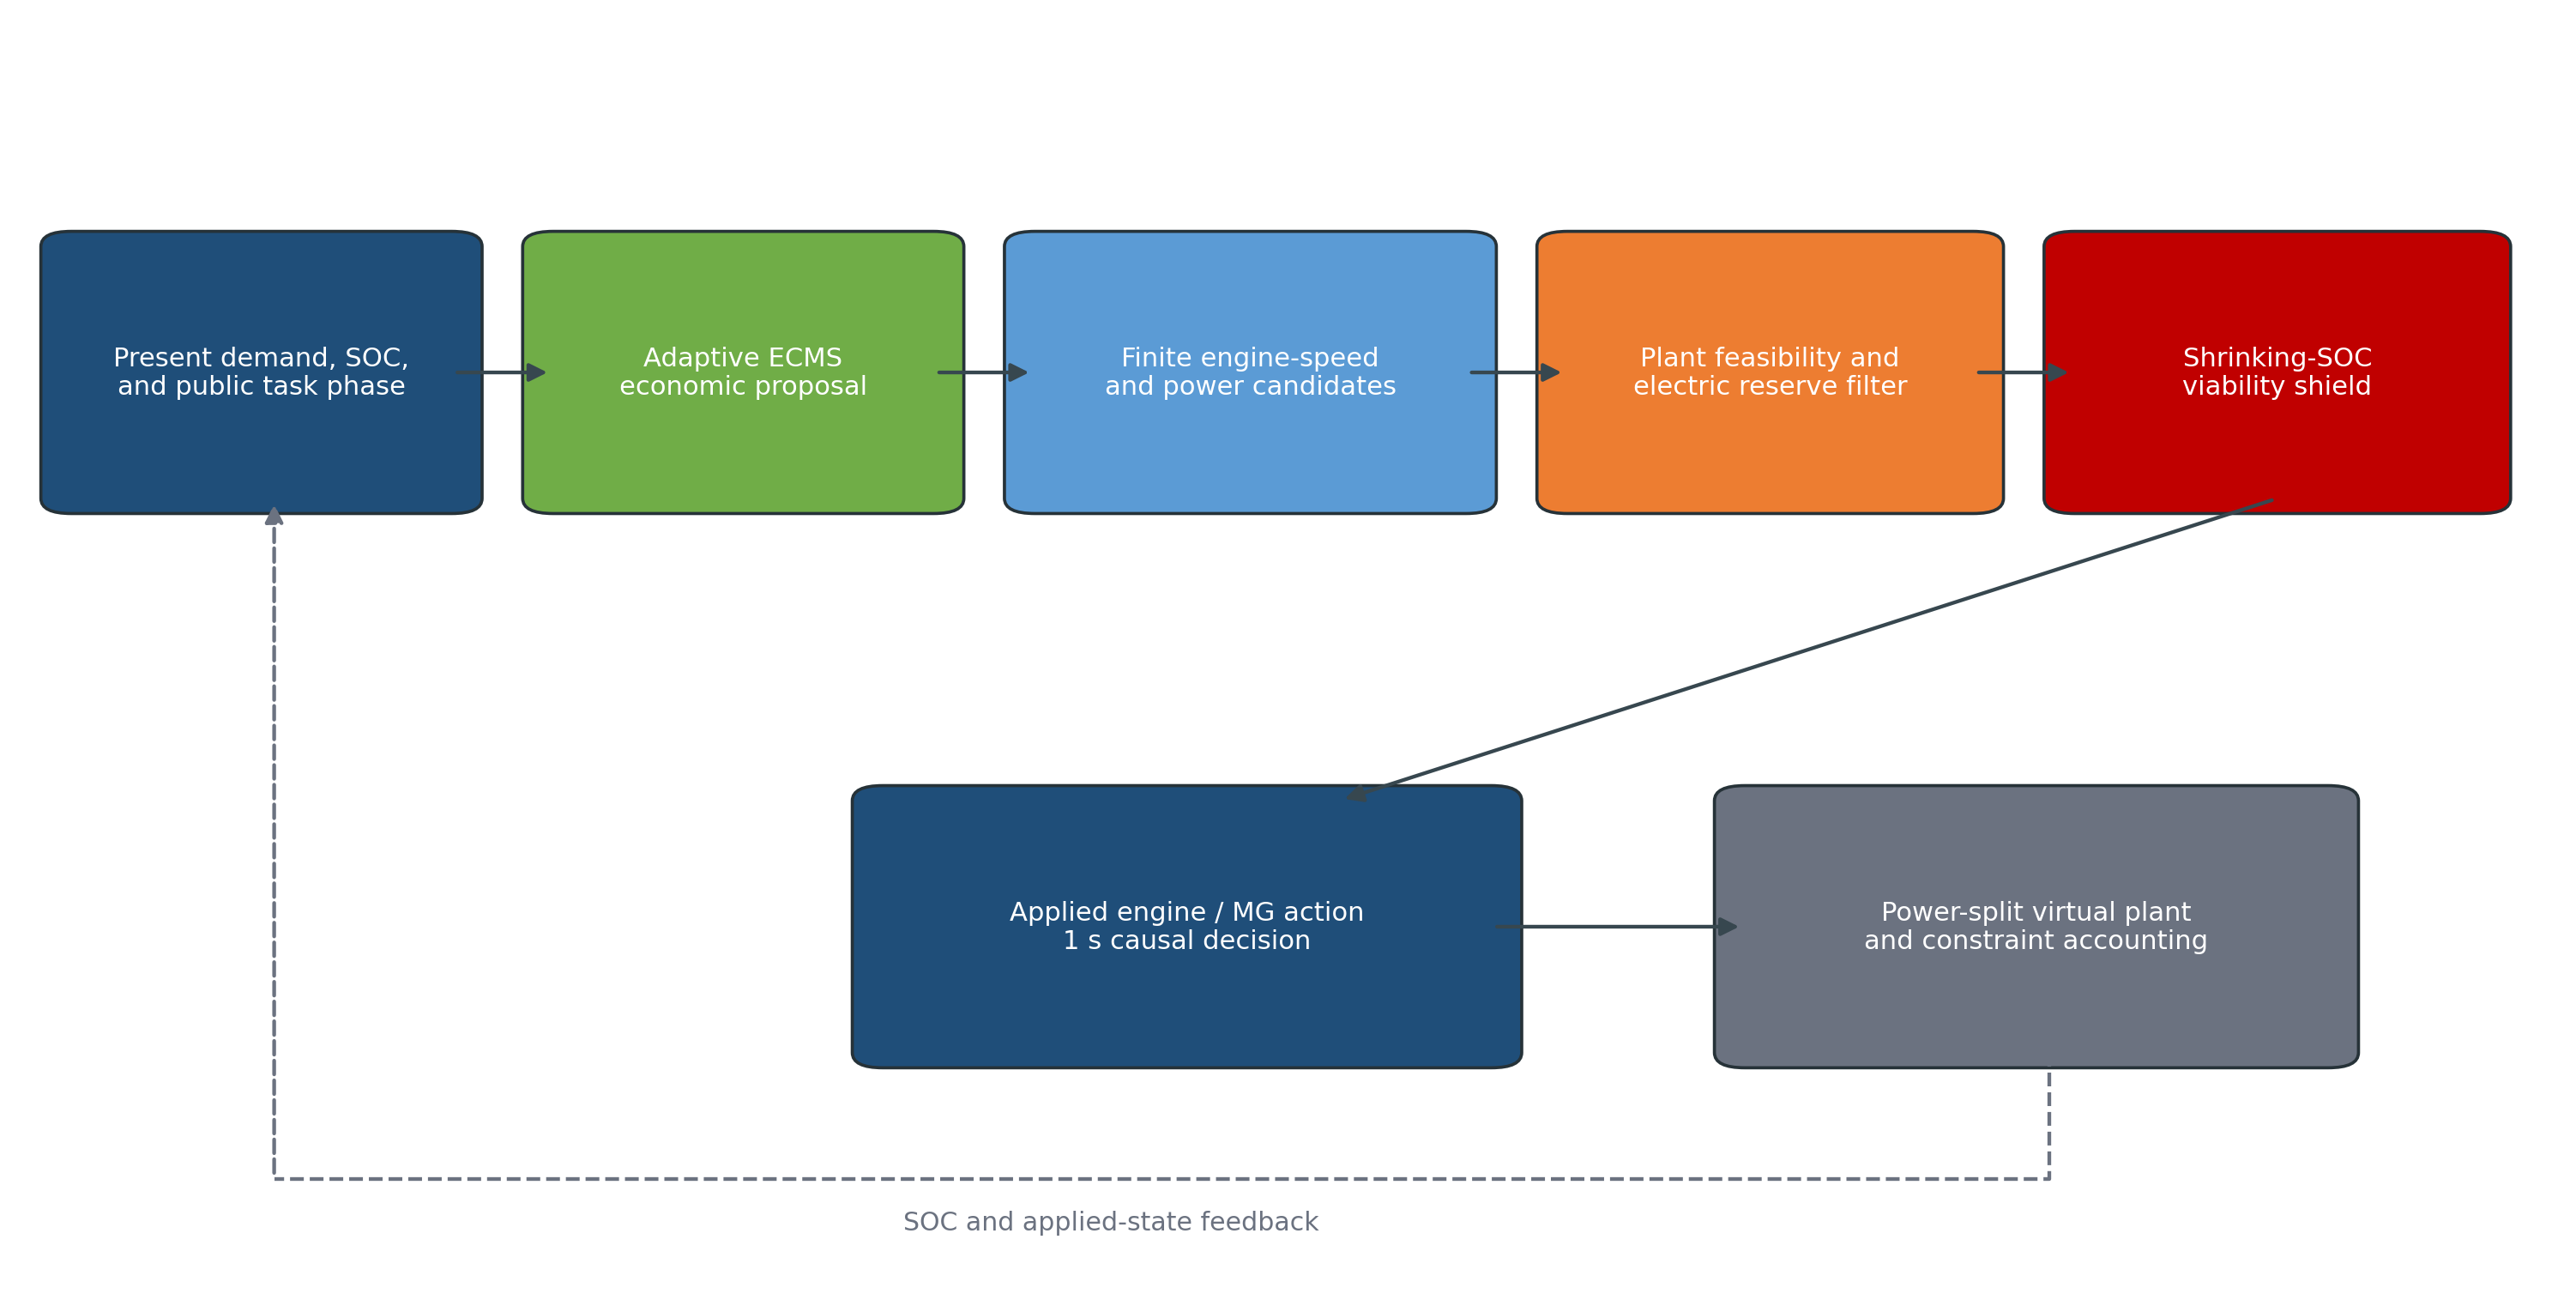
\includegraphics[width=0.98\linewidth]{paper2_v2_architecture.png}
\caption{Primary V2 causal architecture. Economic selection, plant feasibility, electric reserve, and terminal-SOC viability are applied inside the controller; the runner does not append a terminal command.}
\label{fig:architecture}
\end{figure}

\subsection{Protocols and validity rule}
The legacy controller-framework comparison uses a 0.1 s sample time, a 600 s stochastic agricultural cycle, and $SOC_0=0.55$. Its common virtual platform has a 300 kW engine, a 200 kWh battery, 150 kW motor and battery-bus limits, a 60 kW stable engine-power floor, and a 40 kW s$^{-1}$ applied engine-power ramp. The engineering out-of-the-loop (OOL) baseline uses the same accessory demand, terminal governor, and plant constraints as every legacy online controller. A legacy run is strictly valid only when $|SOC_T-SOC_0|\le10^{-4}$, maximum traction shortage is no more than 1 W, and motor, battery-bus, proxy MG, speed, and applied-ramp violations are no more than 1 W or rpm. MPC results are additionally certified only when finite-candidate fallback outside the controller and forecast ramp-envelope infeasibility are both zero. Terminal-set MPC must additionally have zero terminal-set violations; its internal safety-filter activations are reported rather than excluded. A low-fuel run outside either rule is not counted as a saving.

The legacy literature-shaped arm uses an engine map derived from the published Deutz BF 6M 2012 C consumption-regression shape \cite{devyanin2023}, rescaled to a 300 kW, 42\% peak-efficiency virtual platform. It is literature-shaped rather than calibrated for a target tractor. A second legacy arm replaces only the engine efficiency shape with a deliberately steep low-load island (efficiency 0.08 at zero load); it retains the same 300 kW platform, cycle, battery, electrical limits, and controller settings. This is a mechanism sensitivity, not a robustness or hardware-validation test.

The stochastic disturbance scale is 0.25 and its 10 s random-walk targets are continuously interpolated, consistent with the actuator-rate limit. The legacy comparison uses seeds 2200--2205 for development and 2220--2239 for testing. The V2 development set uses seeds 3100--3105; its frozen holdout uses 3120--3139, with no test-set parameter selection. The V2 primary protocol uses a 1 s decision interval, 5 kW engine-power actions, 180 kW MG1/MG2 and battery-bus limits, a 200 kWh battery, a 5 s minimum on dwell, a one-sample minimum off dwell, and a $10^{-3}$ engineering terminal-SOC tolerance. The independent strict audit repeats the frozen controller at $10^{-4}$ without changing its gains. All V2 direct-fuel comparisons use same-seed load-following baselines subject to the same start, dwell, reserve, component, and terminal-energy rules; every V2 terminal correction is internal to the controller.

All 33 V2 plant and controller settings are exported directly from the frozen dataclasses to \texttt{paper2\_v2\_parameter\_manifest.csv}, including units, model roles, source class, and sensitivity or selection coverage. Every row is labelled as a researcher-defined theoretical virtual input rather than a measured component specification.

The V2 cross-cycle audit uses new stochastic seeds 3160--3179; action-grid checks use 3180--3185 at 10, 5, and 2.5 kW; map and battery-capacity audits use 3200--3219. None of these paths participates in controller selection. The deterministic, low-load, and stochastic cross-cycle cases use the same 180 kW electrical limits and strict $10^{-4}$ SOC rule. The high-variability case and every map/capacity path are retained even when no ramp-constrained action exists.

For the legacy controller framework, a separate cross-cycle audit used 20 seeds (2026--2045), the literature-shaped map, the common 18 kW accessory load, terminal-SOC tolerance $10^{-4}$, and no offline SOC reference. It evaluated the deterministic agricultural work cycle, the stochastic agricultural cycle, and a high-variability cycle with the engineering OOL, map-aware ECMS, and terminal-set MPC. The audit was not used to retune a controller. A cycle was reported as invalid when the common battery-power or other hard constraint failed; invalid paths were not converted into fuel-saving pairs.

\subsection{Predeclared MPC mechanism map}
The frozen framework comparison identifies one implementation point, but cannot establish whether its fuel result is specific to horizon or forecast information. A separate, predeclared mechanism map therefore uses new development seeds 2400--2405 and new holdout seeds 2420--2439. It evaluates terminal-set scenario MPC at horizons $H=4,8,12$ under two causal information conditions: a history-only predictor, and the same predictor augmented by the public zero-disturbance task phase and the present demand measurement. The phase condition contains no future realization from an evaluated seed. The scenario count, terminal weight, 300 kW platform, two maps, dynamic OOL baseline, $10^{-4}$ SOC rule, and all hard limits are unchanged.

Within each map, only settings certified on all six development paths are eligible; the eligible setting with the greatest mean direct-fuel saving is frozen and evaluated once on all 20 holdout paths. Certification additionally requires zero fallback outside the controller, zero forecast ramp-envelope infeasibility, and zero terminal-set violations. Internal safety-filter activations and elapsed runtime are retained as outcome measures, not used to exclude a path. All six development cells are reported, so the holdout result cannot be interpreted as a post hoc choice of a favorable horizon or preview policy.

Two additional frozen sensitivity audits test virtual inputs that otherwise could be mistaken for hidden sources of the negative result. The first uses 12 new seeds (2500--2511) and changes battery capacity only (120, 200, and 280 kWh), retaining the 150 kW motor/bus limits, literature-shaped map, ECMS factor $\lambda=2.0$, and terminal-set MPC $H=8$ with five scenarios. The second retains the 200 kWh platform and changes only the causal predictor's residual-persistence gain (0, 0.5, and 1.0). Neither capacity nor gain is selected by its outcome. For every online decision, the implementation records wall-clock time from causal prediction through candidate selection, safety projection, and terminal-energy correction. These local Python timings characterize the finite-set implementation only; they are not an embedded real-time certification.

\section{Results}
\subsection{V2 frozen viability-shielded ECMS results}
The development scan selected $\lambda_0=1.0$, $K_p=40$, and a public-corridor width of 0.045 SOC units. Candidate selection first required all six development paths to remain strictly valid, then capped mean shield interventions at 100 per path before maximizing development saving. These values were frozen before the 20 holdout paths. The V2 controller was strictly valid on 20/20 holdout paths, with a mean direct fuel saving of 5.675\% and a mean terminal-energy-normalized saving of 5.676\% (95\% CI: 5.122\%--6.230\%). The maximum absolute terminal SOC error was $5.52\times10^{-5}$ under the strict audit. The viability shield activated 93.5 times per 600 s path on average; these activations are reported controller actions rather than hidden repairs. The maximum observed local Python decision time was 2.33 ms in the primary run and 9.50 ms in the strict rerun, illustrating wall-clock jitter.

\begin{table}[H]
\centering
\caption{Frozen V2 holdout results on 20 new stochastic cycles. Values are paired with the same-seed load-following baseline.}
\label{tab:v2-main}
\scriptsize
\resizebox{\textwidth}{!}{%
\begin{tabular}{lrrrrr}
\toprule
Method & Strict valid & Mean saving (\%) & 95\% CI (\%) & Max $|\Delta SOC|$ & Max decision (ms) \\
\midrule
V2 viability-shielded adaptive ECMS & 20/20 & 5.676 & 5.122--6.230 & $5.52\times10^{-5}$ & 2.33 \\
V2 strict $10^{-4}$ audit & 20/20 & 5.676 & 5.122--6.230 & $5.52\times10^{-5}$ & 9.50 \\
\bottomrule
\end{tabular}
}
\end{table}

Independent cross-cycle tests retained positive energy-normalized savings of 5.613\% on the deterministic work cycle, 7.954\% on the low-load cycle, and 5.386\% on 20 additional stochastic paths (20/20 valid; minimum 2.597\%). The high-variability cycle produced an empty electrical action set and is therefore reported as a platform-demand boundary, not converted into a fuel statistic.

\begin{figure}[H]
\centering
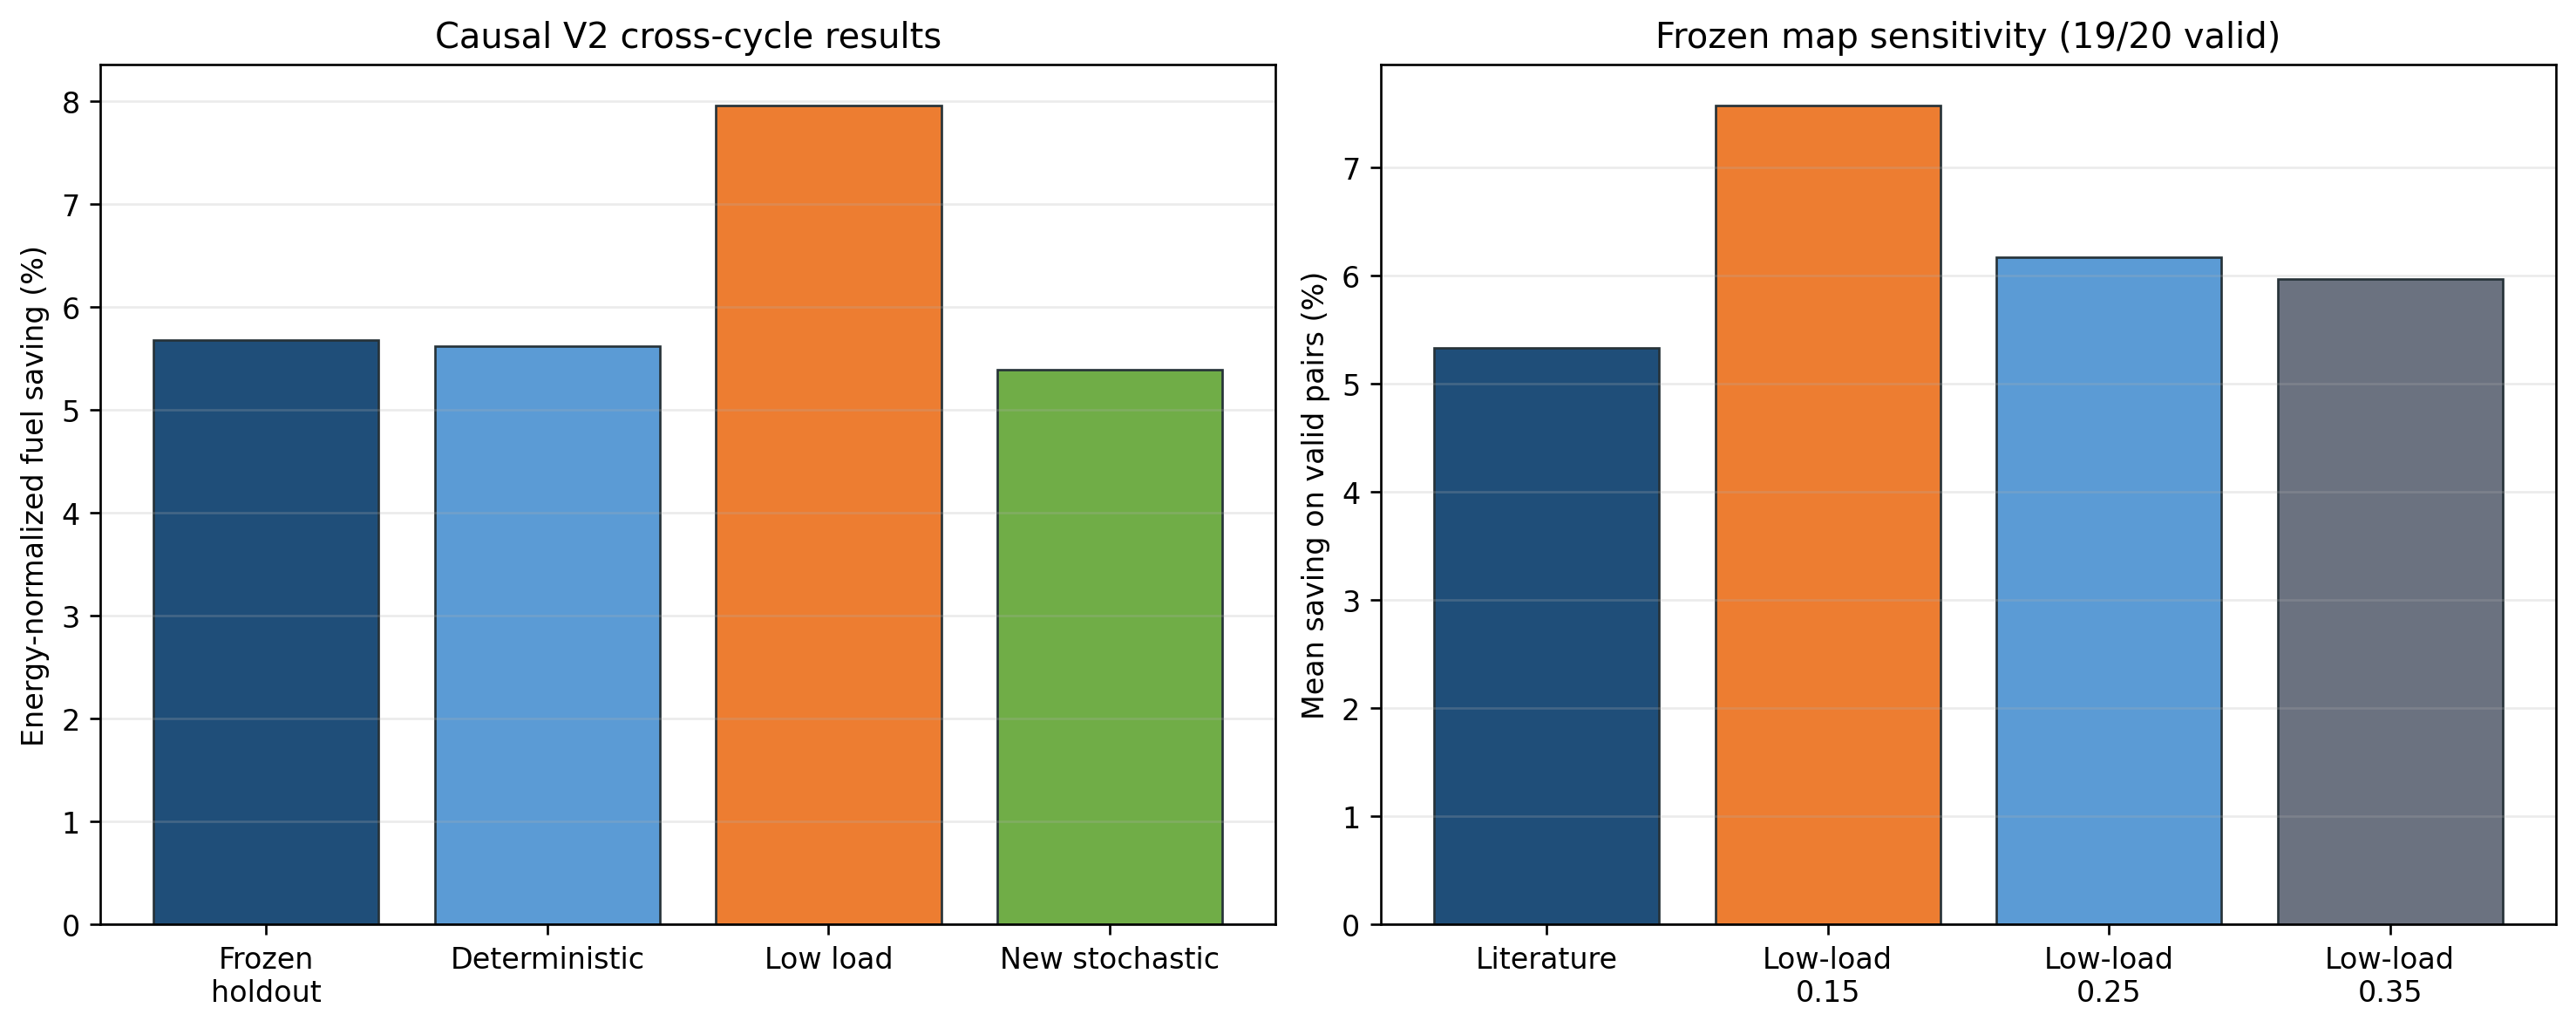
\includegraphics[width=0.98\linewidth]{paper2_v2_results.png}
\caption{Frozen V2 fuel results across independent cycles (left) and engine-map sensitivities (right). Map means include only declared valid pairs, while the common invalid path remains in the validity count.}
\label{fig:v2-energy-results}
\end{figure}

\subsection{V2 map, capacity, and action-grid audits}
With no retuning, the literature-shaped map gave 19/20 valid paths and 5.336\% mean saving. Low-load efficiency settings of 0.15, 0.25, and 0.35 gave 7.576\%, 6.172\%, and 5.969\% on their valid 19/20 pairs. Battery capacities of 120, 200, and 280 kWh gave 3.684\%, 5.336\%, and 5.811\%, respectively. The same high-demand path was invalid because its applied engine-ramp and electrical constraints produced no feasible action; it is retained as a platform-demand failure boundary. Reducing the action grid from 10 to 5 to 2.5 kW changed the six-seed mean to 5.050\%, 5.120\%, and 4.740\%, with 6/6 valid at each resolution. Thus, the saving direction is stable, while the 5 kW value retains an explicit discretization-sensitivity limitation.

\subsection{Legacy strict controller-framework comparison}
All test-set OOL runs and all certified controller pairs met the $10^{-4}$ terminal-SOC rule. On the literature-shaped map, the phase policy was the only controller with a positive mean, but its $0.010\%$ saving is practically negligible. Frozen map-aware ECMS increased fuel use by $0.251\%$. Deterministic MPC was strictly valid on 15/20 runs and zero-fallback certified on 8/20; scenario MPC was strictly valid on 20/20 and certified on 18/20. The terminal-set scenario MPC was strictly valid and zero-external-fallback certified on all 20 paths, with zero terminal-set violations; its internal safety filter activated 614 times (30.7 per path). Its paired fuel change was $-0.704\%$. The result closes the finite-candidate feasibility gap without concealing the intervention frequency, but the additional conservatism does not improve fuel use.

The steep-island sensitivity reverses only the ECMS result: the frozen factor $\lambda=2.0$ saved $10.491\%$ on all 20 pairs. The phase policy and all MPC variants remained fuel-inferior. Terminal-set MPC again achieved 20/20 strict and zero-external-fallback certifications with zero terminal-set violations, while its filter activated 619 times (31.0 per path) and its fuel change was $-3.219\%$. Because all virtual hardware, cycle, terminal-energy rule, and test seeds are unchanged, the contrast identifies the assumed engine-efficiency shape as the source of this virtual benefit; it does not imply a field fuel saving.

\begin{table}[H]
\centering
\caption{Strictly causal 20-seed controller comparison. Direct-fuel statistics use only strict-terminal-SOC and, for MPC, certified pairs with no fallback outside the controller. Terminal-set MPC additionally has zero terminal-set violations; its safety-filter activations are reported rather than treated as excluded samples. All values are paired with the same-seed engineering OOL.}
\label{tab:framework}
\scriptsize
\setlength{\tabcolsep}{3pt}
\begin{tabular}{llrrrl}
\toprule
Engine map & Controller & Strict valid & Certified pairs & Filter steps & Saving vs. OOL (\%) \\
\midrule
Literature-shaped & Map-aware ECMS & 20/20 & 20 & -- & $-0.251$ [$-0.264$, $-0.238$] \\
Literature-shaped & Nominal phase policy & 20/20 & 20 & -- & $+0.010$ [$+0.006$, $+0.015$] \\
Literature-shaped & Deterministic MPC & 15/20 & 8 & -- & $-0.658$ [$-0.700$, $-0.615$] \\
Literature-shaped & Scenario MPC & 20/20 & 18 & -- & $-0.346$ [$-0.374$, $-0.319$] \\
Literature-shaped & Terminal-set scenario MPC & 20/20 & 20 & 614 & $-0.704$ [$-0.756$, $-0.653$] \\
\midrule
Steep-island sensitivity & Map-aware ECMS & 20/20 & 20 & -- & $+10.491$ [$+10.445$, $+10.538$] \\
Steep-island sensitivity & Nominal phase policy & 20/20 & 20 & -- & $-0.077$ [$-0.133$, $-0.021$] \\
Steep-island sensitivity & Deterministic MPC & 15/20 & 8 & -- & $-2.213$ [$-2.292$, $-2.133$] \\
Steep-island sensitivity & Scenario MPC & 20/20 & 18 & -- & $-2.529$ [$-2.785$, $-2.273$] \\
Steep-island sensitivity & Terminal-set scenario MPC & 20/20 & 20 & 619 & $-3.219$ [$-3.884$, $-2.553$] \\
\bottomrule
\end{tabular}
\end{table}

\subsection{Frozen storage and causal-forecast sensitivities}
Table~\ref{tab:store-forecast} reports the independent 12-seed audits. Changing battery capacity from 120 to 280 kWh did not change the strict-valid or certified rate: ECMS and terminal-set MPC were certified on all pairs, but both remained fuel-inferior. The terminal-set MPC fuel change ranged from $-0.732\%$ to $-0.501\%$; the fixed ECMS result remained $-0.275\%$. Thus, the primary negative MPC result is not explained by the single 200 kWh energy-capacity input within this declared family.

Likewise, causal residual persistence did not recover a positive MPC result. It changed the mean number of safety projections from 37.25 to 0.42 per path, but the fuel change remained between $-0.690\%$ and $-0.725\%$. This is evidence about the three declared predictor settings rather than a universal forecast-robustness result. Across these executions, the largest per-run P95 decision time was 1.71 ms and the largest observed individual local Python decision was 84.39 ms, both below the 100 ms simulation sample interval. These timing figures include the finite candidate search and safety projection, but are deliberately not used as evidence of embedded implementation readiness.

\begin{table}[H]
\centering
\caption{Frozen virtual storage and causal-forecast sensitivity audit on 12 new seeds. Negative saving denotes increased fuel use relative to the same-seed dynamic OOL. No row was used for retuning.}
\label{tab:store-forecast}
\scriptsize
\setlength{\tabcolsep}{3pt}
\begin{tabularx}{\linewidth}{@{}X l r r r@{}}
\toprule
Audit & Controller & Certified & Saving vs. OOL (\%) & Mean filter steps/path \\
\midrule
120 kWh battery & ECMS & 12/12 & $-0.275$ & 0.00 \\
120 kWh battery & Terminal-set MPC & 12/12 & $-0.732$ & 37.00 \\
200 kWh battery & ECMS & 12/12 & $-0.275$ & 0.00 \\
200 kWh battery & Terminal-set MPC & 12/12 & $-0.690$ & 37.25 \\
280 kWh battery & ECMS & 12/12 & $-0.275$ & 0.00 \\
280 kWh battery & Terminal-set MPC & 12/12 & $-0.501$ & 34.67 \\
Residual gain 0.0 & Terminal-set MPC & 12/12 & $-0.690$ & 37.25 \\
Residual gain 0.5 & Terminal-set MPC & 12/12 & $-0.709$ & 4.08 \\
Residual gain 1.0 & Terminal-set MPC & 12/12 & $-0.725$ & 0.42 \\
\bottomrule
\end{tabularx}
\end{table}

\begin{figure}[H]
\centering
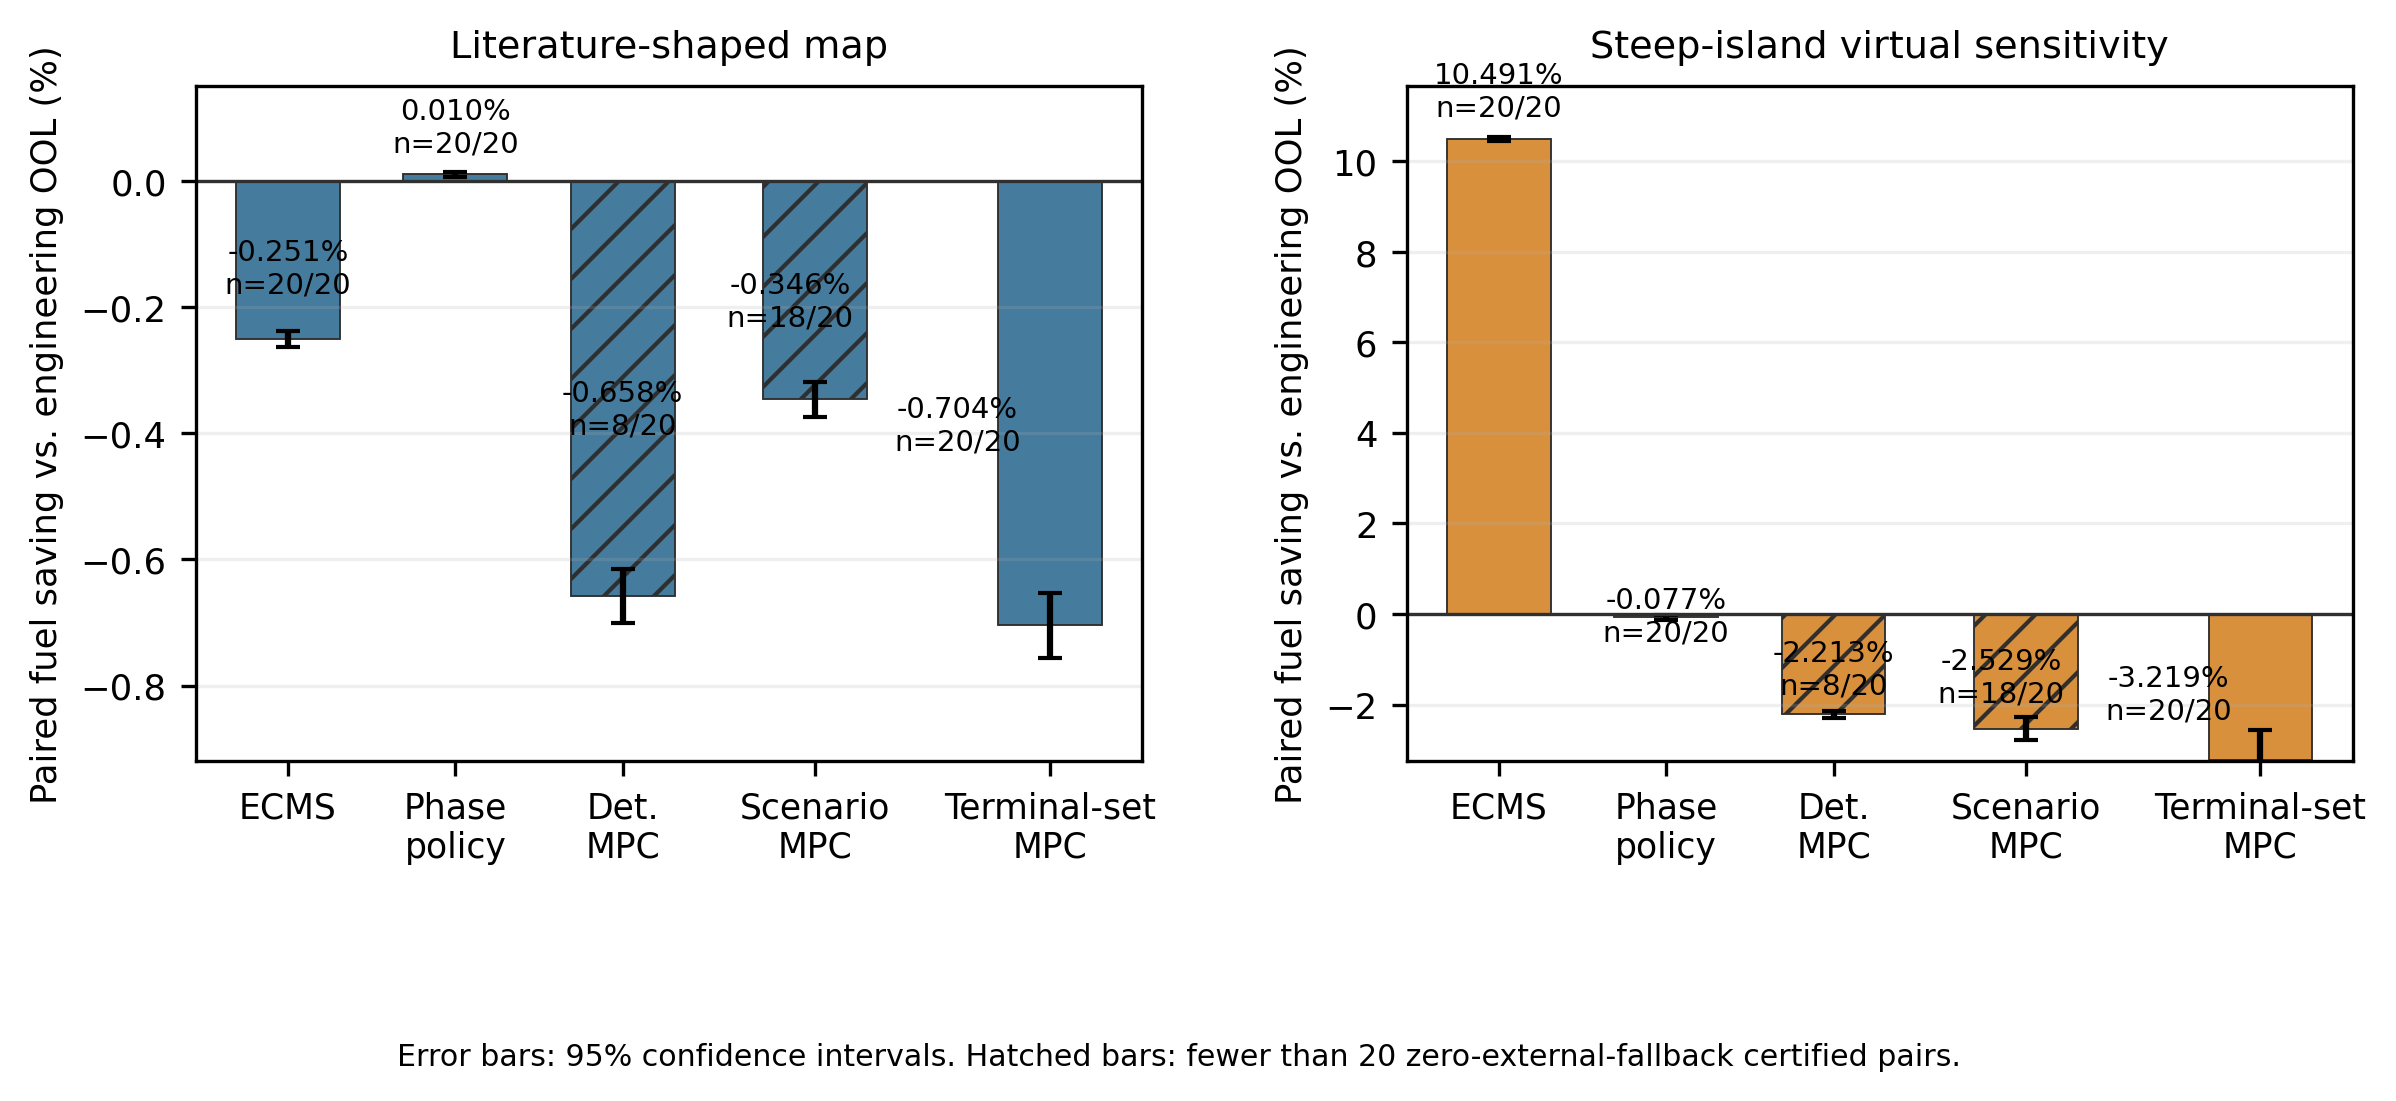
\includegraphics[width=0.98\linewidth]{paper2_controller_framework.png}
\caption{Frozen strictly causal controller comparison on the 20 unseen stochastic-cycle seeds. Error bars show 95\% confidence intervals. Hatched MPC bars have fewer than 20 certified pairs with no fallback outside the controller. Terminal-set MPC has 20 certified paths in both panels; its internal filter counts appear in Table~\ref{tab:framework}. The right panel is a declared virtual-map sensitivity, not an engineering-performance estimate.}
\label{fig:framework}
\end{figure}

\subsection{Virtual efficiency-map sensitivity}
The strict framework comparison was complemented by a fixed-controller map sweep to quantify how the low-load efficiency assumption changes the causal ranking. We froze the ECMS factor ($\lambda=2.0$), terminal-set MPC horizon ($H=8$), five causal scenarios, terminal weight, public nominal phase preview, 300 kW platform, and all constraints. Seven low-load efficiency levels from 0.08 to 0.35 were evaluated on 20 new seeds (2260--2279); no level was used to tune a controller. At the steepest virtual map (0.08), map-aware ECMS saved 12.543\% (95\% CI: 12.511--12.575\%), whereas terminal-set MPC increased fuel use by 3.464\% (95\% CI: 2.645--4.282\%). At 0.25, ECMS saved 3.269\% and MPC increased fuel use by 0.918\%; at 0.35, ECMS increased fuel use by 1.075\% and MPC increased fuel use by 0.248\%. The continuous trend is produced by an explicit low-load-island parameterization of both the idle and first-20\% load columns, rather than by clipping higher settings to a base-grid row. Every tested controller pair was strictly valid and certified. Figure~\ref{fig:map-sensitivity} therefore identifies the low-load map shape as a first-order virtual mechanism, while showing that the recursive-feasibility construction does not become fuel-positive within this declared map family.

To test whether the strict $10^{-4}$ terminal-SOC rule alone caused the negative ranking, we repeated the literature-shaped-map protocol at tolerances $10^{-4}$, $5\times10^{-4}$, and $10^{-3}$ on 20 new seeds (2280--2299). All ECMS and terminal-set MPC runs remained strictly valid and certified at every tolerance. ECMS changed by $-0.258\%$ (95\% CI: $-0.281$ to $-0.235\%$), while terminal-set MPC changed by $-0.703\%$ (95\% CI: $-0.765$ to $-0.642\%$) at all three tolerances. The negative MPC result is therefore not removed by this terminal-accounting relaxation within the tested virtual protocol.

\subsection{Independent cross-cycle demand-envelope audit}
Table~\ref{tab:cross-cycle} reports the independent audit using the same strict validity and certification rules. On the deterministic agricultural cycle, all three controllers were certified, but ECMS and terminal-set MPC increased fuel by 0.431\% and 0.137\%, respectively. On the stochastic agricultural cycle, terminal-set MPC remained certified on all 20 seeds and increased fuel by 0.768\%; ECMS was strictly valid on 14/20 seeds and its valid pairs increased fuel by 0.391\%. The high-variability cycle exceeded the current virtual battery-power envelope on all 20 seeds for all three controllers. Those paths are deliberately reported as a platform-demand boundary, not removed from the audit and not used to imply a controller advantage.

\begin{table}[H]
\centering
\caption{Independent cross-cycle demand-envelope audit on the literature-shaped virtual map. Negative values denote fuel increases relative to the same-seed engineering OOL. A dash indicates that no strict-valid pair exists.}
\label{tab:cross-cycle}
\scriptsize
\setlength{\tabcolsep}{3pt}
\begin{tabular}{llrrr}
\toprule
Cycle & Controller & Strict valid & Certified & Saving vs. OOL (\%) \\
\midrule
Agricultural & Engineering OOL & 20/20 & 20/20 & -- \\
Agricultural & Map-aware ECMS & 20/20 & 20/20 & $-0.431$ \\
Agricultural & Terminal-set MPC & 20/20 & 20/20 & $-0.137$ \\
Stochastic agricultural & Engineering OOL & 20/20 & 20/20 & -- \\
Stochastic agricultural & Map-aware ECMS & 14/20 & 14/20 & $-0.391$ \\
Stochastic agricultural & Terminal-set MPC & 20/20 & 20/20 & $-0.768$ \\
High-variability & Engineering OOL & 0/20 & 0/20 & -- \\
High-variability & Map-aware ECMS & 0/20 & 0/20 & -- \\
High-variability & Terminal-set MPC & 0/20 & 0/20 & -- \\
\bottomrule
\end{tabular}
\end{table}

We then performed a separate capability screen without retuning any controller. The high-variability cycle was shortened to 300 s and evaluated on 12 predeclared seeds while the motor peak and battery-bus limits were changed together from 150 to 225 kW. At 175 kW, the engineering OOL and terminal-set MPC became valid on all 12 paths, but ECMS remained invalid; at 200 kW the same pattern remained. At 225 kW all three controllers were valid, while terminal-set MPC still increased fuel by 0.320\% and ECMS increased fuel by 0.468\% relative to the matched OOL. This capability screen therefore identifies an admissible virtual demand boundary rather than a hidden controller tuning opportunity (Table~\ref{tab:power-boundary}).

\begin{table}[H]
\centering
\caption{High-variability capability screen with paired motor-peak and battery-bus limits. The 12 seeds and 300 s cycle were frozen before the screen; negative savings denote fuel increases.}
\label{tab:power-boundary}
\scriptsize
\setlength{\tabcolsep}{3pt}
\begin{tabular}{rrrrr}
\toprule
Paired limit (kW) & OOL valid & ECMS valid & Terminal-set MPC valid & Valid-pair saving (\%) \\
\midrule
150 & 0/12 & 0/12 & 0/12 & -- \\
175 & 12/12 & 0/12 & 12/12 & $-0.283$ (MPC) \\
200 & 12/12 & 0/12 & 12/12 & $-0.334$ (MPC) \\
225 & 12/12 & 12/12 & 12/12 & $-0.468$ (ECMS), $-0.320$ (MPC) \\
\bottomrule
\end{tabular}
\end{table}

\begin{figure}[H]
\centering
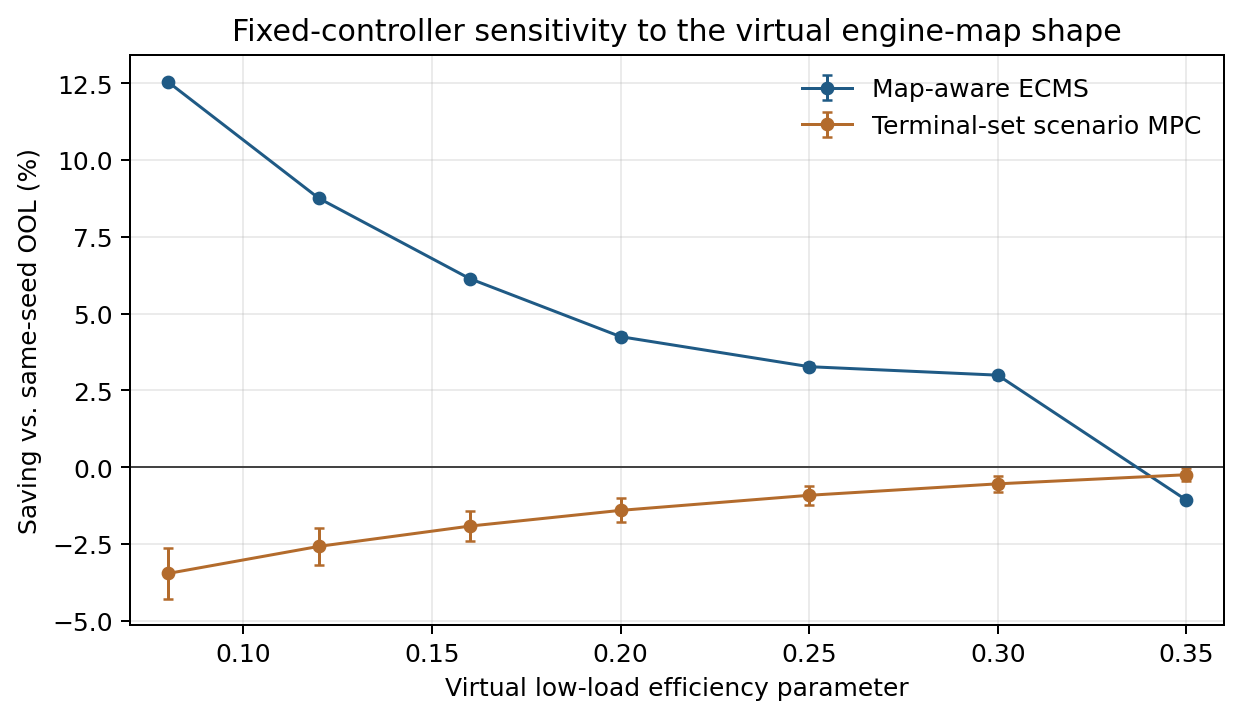
\includegraphics[width=0.92\linewidth]{paper2_map_sensitivity_grid.png}
\caption{Fixed-controller sensitivity to the virtual low-load efficiency parameter on 20 independent seeds per level. Error bars are 95\% confidence intervals. The ECMS factor, MPC horizon, causal information set, terminal-SOC rule, and hardware limits were frozen before the sweep.}
\label{fig:map-sensitivity}
\end{figure}

\subsection{Horizon--preview mechanism map}
Figure~\ref{fig:mechanism} rules out a positive terminal-set MPC result as an artifact of the original eight-sample, public-phase setting within the declared mechanism grid. On the literature-shaped map, history-only $H=8$ was the best eligible development setting ($-0.171\%$) and was frozen. Its 20/20 certified holdout result was $-0.168\%$ (95\% CI: $-0.190$ to $-0.146\%$), with no safety-filter activations. The public-phase variants were more fuel-inferior and activated the filter 13.5--34.5 times per development path. History-only $H=4$ was certified on only one of six development paths.

The same selection occurred on the steep-island map: history-only $H=8$ was the closest eligible development setting to OOL ($-2.034\%$), yet its independent 20/20 holdout result was $-2.079\%$ (95\% CI: $-2.106$ to $-2.051\%$), with no filter activations. Increasing the horizon or adding the public phase did not yield a positive certified result; phase-preview $H=12$ was certified on only five of six development paths. The screen is not a claim about all MPC formulations or all cycle classes. It establishes, for the six prespecified causal settings and two declared maps, that forecast information and a longer finite horizon did not recover a fuel advantage after strict terminal-energy and feasibility accounting.

\begin{figure}[H]
\centering
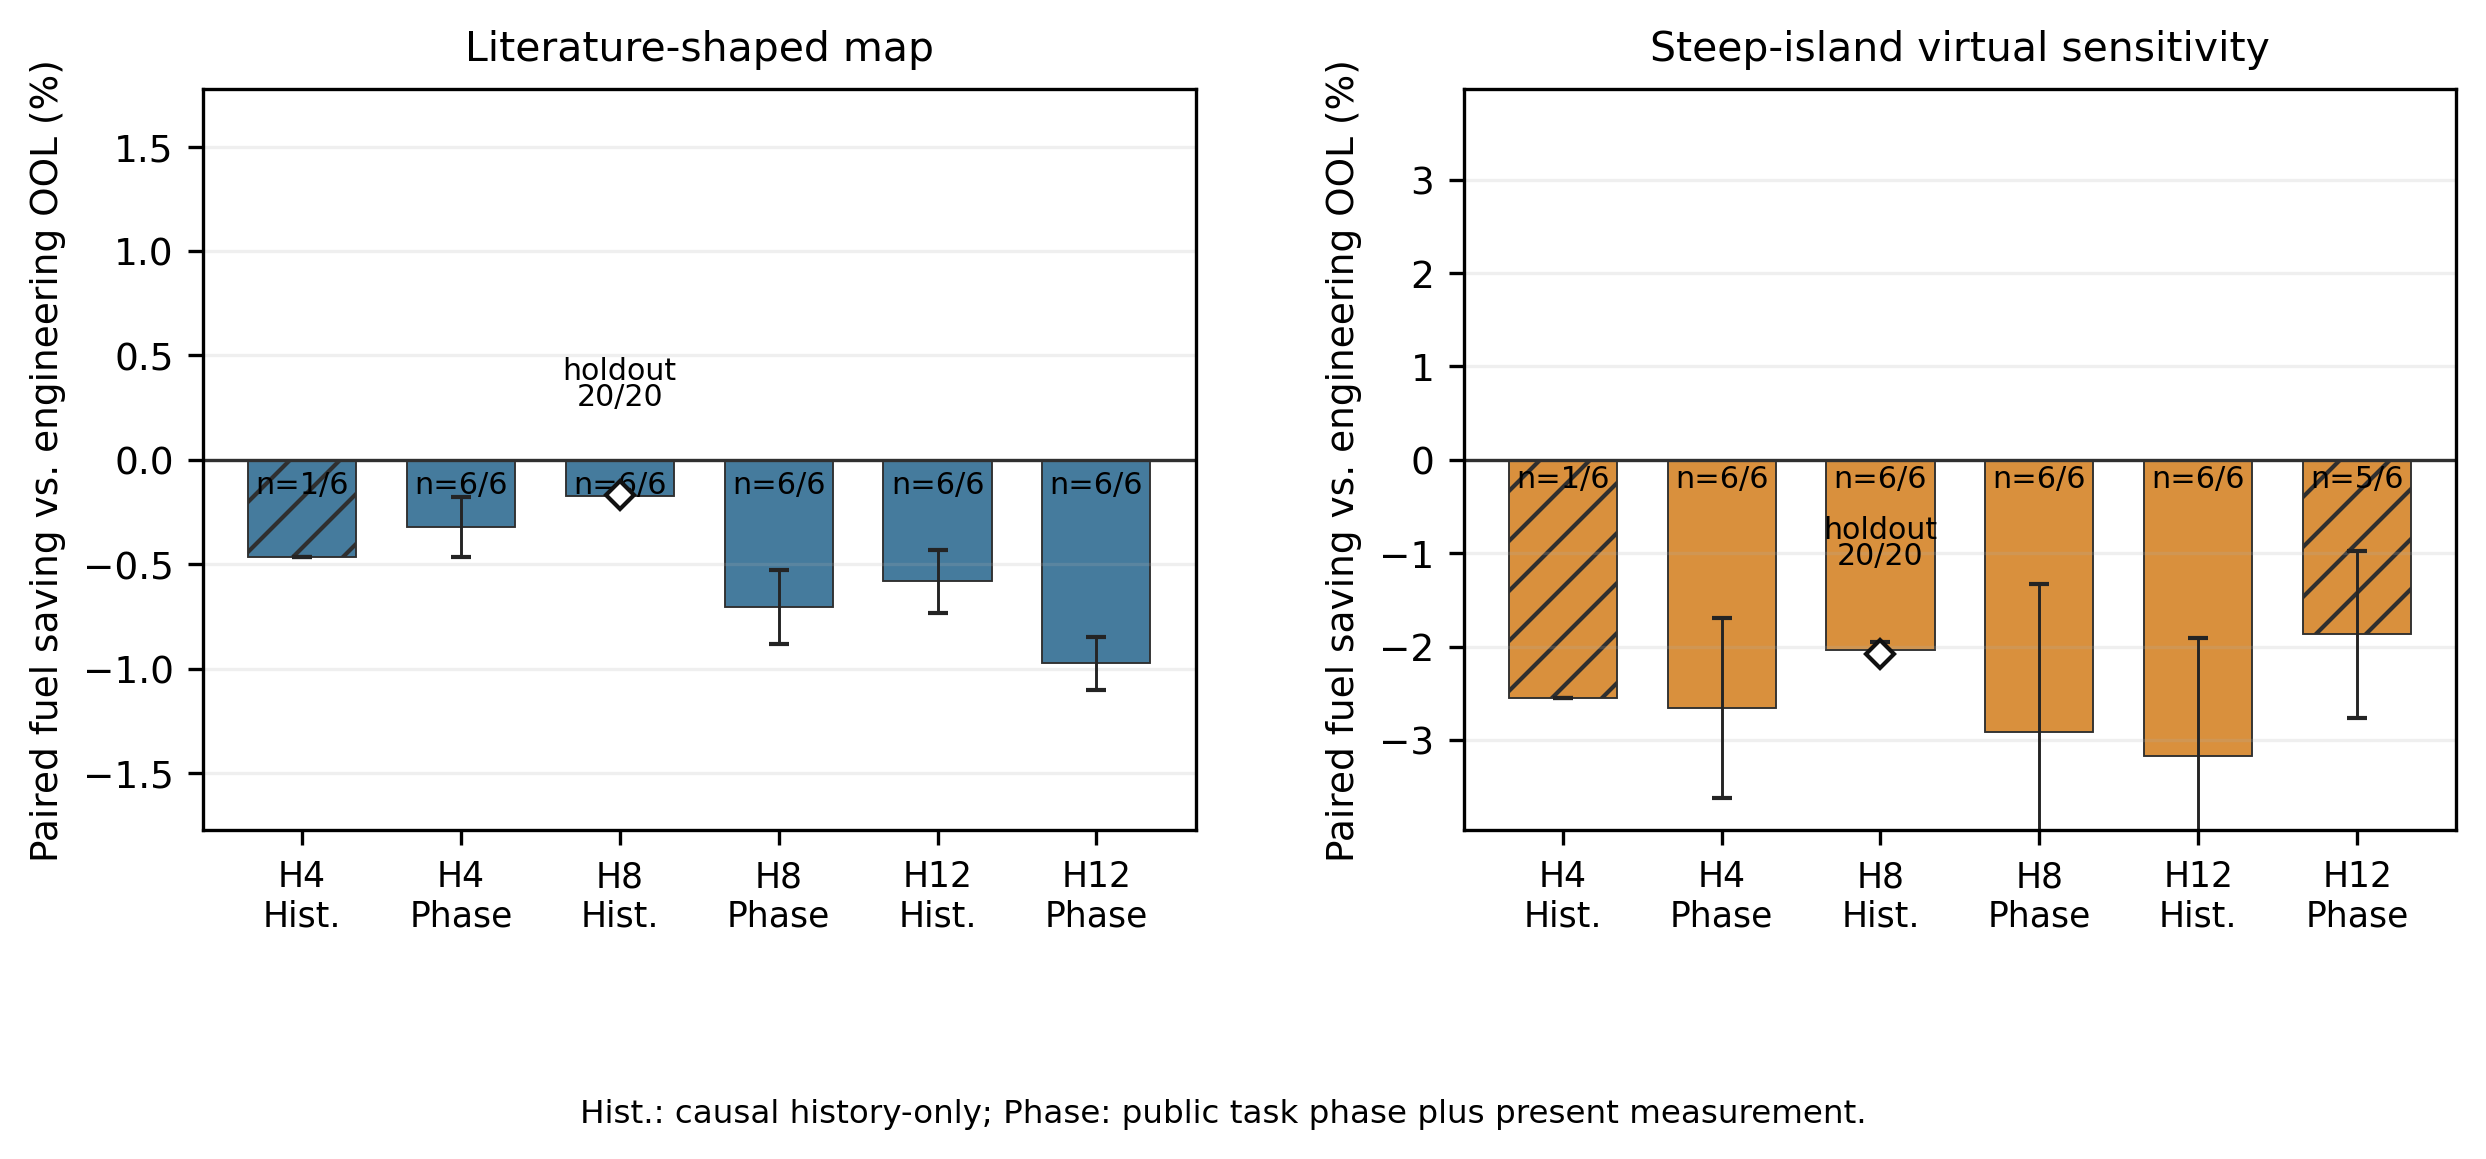
\includegraphics[width=0.98\linewidth]{paper2_mpc_mechanism_map.png}
\caption{Predeclared horizon--preview mechanism map for terminal-set scenario MPC. Bars are six-path development means with 95\% confidence intervals. Hatched bars have fewer than six certified paths. The diamond is the setting selected solely on development results and then evaluated on 20 disjoint holdout paths. ``Hist.'' uses only causal history and the present measurement; ``Phase'' adds the public nominal task phase, but no realized future sample.}
\label{fig:mechanism}
\end{figure}

\begin{table}[H]
\centering
\caption{Independent holdout check of the development-selected mechanism-map setting. The negative values are reported as fuel increases relative to the same-seed engineering OOL; they are retained to quantify the feasibility--fuel trade-off rather than suppressed.}
\label{tab:mechanism-holdout}
\scriptsize
\setlength{\tabcolsep}{3pt}
\begin{tabularx}{\linewidth}{@{}X p{0.27\linewidth} p{0.13\linewidth} p{0.30\linewidth}@{}}
\toprule
Virtual map & Development-frozen setting & Holdout (n/20) & Saving vs. OOL (\%, 95\% CI) \\
\midrule
Literature-shaped & $H=8$, history-only & 20/20 & $-0.168$ [$-0.190$, $-0.146$] \\
Steep-island sensitivity & $H=8$, history-only & 20/20 & $-2.079$ [$-2.106$, $-2.051$] \\
\bottomrule
\end{tabularx}
\end{table}

\subsection{Idealized full-information envelope}
A separate, predeclared oracle diagnostic quantifies how much favorable virtual-model headroom remains when the complete future of the smooth nominal task is known. It retains the same 300 kW platform, 200 kWh battery, 150 kW motor and battery-bus limits, 60 kW stable engine floor, 40 kW s$^{-1}$ applied ramp, wheel-side recovery, physical SOC bounds, and dynamic realistic-OOL baseline. Its only intentional idealizations are full future information and a task-level terminal SOC band of $\pm0.01$, rather than the $10^{-4}$ direct-fuel rule used above. It is therefore not included in the causal controller comparison.

Both declared map conditions were evaluated at 4 kW/0.005-SOC and 2 kW/0.002-SOC grid resolutions. The literature-shaped grid solution was rejected after continuous replay, which ended at a SOC error of $-0.0310$ and thus exceeded the declared task-level band. Under the deliberately steep low-load map, the continuous 4 kW trajectory met all hard limits and ended at a SOC error of $+0.00669$; the refined-grid raw value differed by only 0.004 percentage points. Its continuous-replay raw engine-fuel reduction was 21.611\%. However, the paired OOL ended at $+0.00950$ SOC, leaving the oracle 0.563 kWh lower. Returning that energy at a predeclared 0.42 fuel-conversion efficiency adds 0.136 L, giving an energy-normalized reduction of 19.828\%, i.e., approximately 20\% only in this idealized full-information virtual case (Table~\ref{tab:oracle}).

\begin{table}[H]
\centering
\caption{Declared full-information oracle diagnostic. These values are excluded from the strictly causal controller statistics. The raw result is shown with terminal-energy normalization so that a task-level SOC band is not mistaken for a directly comparable fuel saving.}
\label{tab:oracle}
\scriptsize
\setlength{\tabcolsep}{3pt}
\begin{tabularx}{\linewidth}{@{}X p{0.23\linewidth} p{0.14\linewidth} p{0.20\linewidth}@{}}
\toprule
Virtual map & Continuous result & Raw saving (\%) & Normalized saving (\%) \\
\midrule
Literature-shaped & Rejected ($\Delta SOC=-0.0310$) & -- & -- \\
Steep low-load sensitivity & All hard limits satisfied & $+21.611$ & $+19.828$ \\
\bottomrule
\end{tabularx}
\end{table}

\subsection{Excluded full-information diagnostics}
Earlier full-future dynamic-programming and looser-terminal-SOC explorations are retained in the reproducibility archive as diagnostic audits only. They are excluded from this article's online comparison because full future demand, grid-terminal feasibility, or residual terminal battery energy can produce fuel figures that are not available to a causal controller. In particular, a former 24.087\% grid value failed continuous SOC replay and is not reported as a result. The causal controller statistics above use the common $10^{-4}$ terminal-SOC threshold exclusively.

\section{Discussion}
The V2 result changes the central interpretation of the study. A causal controller can obtain a positive fuel result when the economic objective and terminal-energy protection are implemented in one controller, rather than when a short-horizon MPC is followed by a common external correction. The 5.68\% normalized saving survives the $10^{-4}$ audit, new stochastic paths, deterministic and low-load cycles, and the declared map/capacity family. The positive result is conditional on the public task-phase SOC corridor, the 5 kW action grid, the virtual component maps, and the stated electrical envelope; it is not a hardware fuel-economy estimate.

The V2 safety shield is active rather than cosmetic: its average 93.5 actions per path and the single invalid high-demand path expose how often the economic proposal conflicts with charge-sustaining feasibility. The added cold-start, minimum-dwell, and 35\% electric-headroom rules prevent the controller from depending on an instantaneous high-power restart after shutdown. This makes the controller more auditable than a post-processing correction, but it also means the method should be described as a discrete viability-shielded ECMS rather than as an unconstrained ECMS optimum. The intervention-cap selection reduces the mean action count without removing the strict SOC screen; the action-grid audit shows that the direction of the saving is stable, while the exact percentage remains discretization-sensitive.

The legacy literature-shaped arm does not support a meaningful fuel-saving effect from its terminal-set MPC. Its negative result is retained as a negative control: it demonstrates that recursive feasibility alone does not imply fuel optimality, and it motivates the V2 separation between economic selection and viability filtering.

The steep-island arm supplies a more informative mechanism result than a controller ranking alone. Its large ECMS effect is achieved without future demand and under the same terminal-energy and hardware rules, but it disappears when the engine map is replaced by the literature-shaped arm. The result therefore attributes the virtual saving to the assumed low-load efficiency penalty and the associated opportunity for load shifting. It must not be interpreted as an estimate for a physical tractor, and it would be inappropriate to select the 10.491\% number as a headline performance result.

The horizon--preview map separates the central negative result from a single arbitrary MPC setting. Both development procedures selected history-only $H=8$, and both independent holdout results remained negative with 20/20 certification. The failure of public-phase variants to improve fuel use is particularly informative: in this finite-set implementation, the additional phase prior caused more safety projections without an offsetting map-aware load-shifting gain. This does not prove that preview is universally detrimental. It bounds the conclusion to the declared horizons, predictor, cycle, virtual maps, and terminal-set construction, while ruling out an unsupported claim that modest causal preview or a longer tested horizon restores MPC fuel savings.

The full-information oracle makes the same distinction from another direction. The approximately 20\% energy-normalized value requires both the declared steep low-load map and future knowledge of the entire smooth nominal task; the literature-shaped counterpart did not survive continuous terminal-SOC replay. It measures virtual headroom, not a causal-controller target. The fixed-map sweep reinforces this interpretation: changing only the low-load efficiency parameter moves ECMS savings from approximately 10.46\% to 3.27\%, while the terminal-set MPC remains fuel-inferior throughout the tested family. Reporting both raw and normalized values is necessary because the task-level terminal band otherwise permits unequal residual battery energy.

An independent strict cross-cycle audit further bounds the claim. With the literature-shaped map, common 18 kW accessory load, terminal-SOC tolerance $10^{-4}$, and no offline SOC reference, all controllers were certified on the deterministic agricultural work cycle, but ECMS and terminal-set MPC increased fuel by 0.431\% and 0.137\%, respectively. On the stochastic agricultural cycle, terminal-set MPC remained certified on all 20 seeds and increased fuel by 0.768\%; ECMS was strictly valid on 14/20 seeds and its valid pairs still increased fuel by 0.391\%. The high-variability cycle exposed a declared platform boundary: all 20 seeds violated the current battery-power envelope, so no fuel-saving claim is made for that cycle. This audit is therefore evidence of conditional feasibility and an explicit demand-envelope limitation, not evidence that the causal MPC generalizes to arbitrary cycles.

The paired-capability screen sharpened this limitation: raising both motor and battery-bus limits to 175 kW restored strict validity for OOL and terminal-set MPC, while ECMS required 225 kW for all 12 screened paths. The restored paths remained fuel-inferior for the causal controllers. Thus, the high-variability result is best interpreted as a declared platform-demand boundary, not as evidence that additional electrical headroom creates an MPC fuel advantage.

The frozen capacity and predictor audits make the component and forecast assumptions more explicit. Across 120--280 kWh, all 12 terminal-set MPC paths per capacity were certified but fuel-inferior; changing causal residual persistence changed safety-filter frequency without changing the sign of the fuel result. These tests do not exhaust virtual battery, motor, or forecast uncertainty, but they rule out two convenient explanations for the reported negative result within a predeclared input family. The recorded decision-time distribution also distinguishes finite-set computational cost from a claim of embedded readiness: local Python timings are reproducible implementation diagnostics, not a latency guarantee for a vehicle controller.

This is a theoretical simulation, so the defined 300 kW component maps, battery model, planetary relation, MG constraints, and stochastic cycle are sufficient inputs for the stated virtual-model findings. The literature-shaped map uses the load trend of a 155 kW Deutz engine only as a transparent reference shape before rescaling; the steep island and the seven-level sweep are deliberately specified mechanism maps. The remaining methodological priorities are broader virtual map families, explicit admissible-demand bounds for the conditional terminal-set guarantee, and a public versioned code/data archive. Real-machine calibration would be a separate study rather than a prerequisite for reproducing or assessing the present theoretical results.

\section{Conclusions}
This study presents a viability-shielded adaptive ECMS for a hybrid-tractor virtual prototype. With no external terminal command repair, the controller achieved 20/20 strict-valid frozen paths and a 5.68\% mean terminal-energy-normalized saving, with positive results on deterministic, low-load, and additional stochastic cycles. Map and battery-capacity audits retained positive savings but exposed one repeatable high-demand empty-action failure; the high-variability cycle also exceeded the declared electrical envelope and was not converted into a saving. The legacy terminal-set MPC comparison remains a negative control showing that feasibility does not by itself imply fuel improvement. The separately reported full-information oracle remains an approximately 20\% headroom diagnostic under an idealized map and relaxed task-level SOC band, not an online or hardware result. All numerical conclusions are therefore conditional on the declared theoretical maps, public task-phase corridor, discrete action grid, start/dwell rules, electric reserve, and virtual power limits.

\authorcontributions{Conceptualization, C.C.; Methodology, C.C.; Software, C.C.; Formal analysis, C.C.; Visualization, C.C.; Writing---original draft preparation, C.C.; Resources, C.C.; Validation, P.W.; Investigation, C.C.; Writing---review and editing, Y.Z.; Supervision, Y.Z.; Project administration, Y.Z.; Funding acquisition, Y.Z.}
\funding{This work has received funding from the Science and Technology Project of the Ministry of Agriculture and Rural Affairs of China.}
\institutionalreview{Not applicable.}
\informedconsent{Not applicable.}
\dataavailability{The V2 virtual-prototype source code, reproduction scripts, parameter manifests, and frozen JSON outputs are provided with the submission as Supplementary Materials. The existing public project archive is available at \url{https://github.com/Fat-pig-Cui/agricultural-tractor-virtual-prototypes}; its version history is indexed by the Zenodo concept DOI \mbox{\href{https://doi.org/10.5281/zenodo.22754509}{10.5281/zenodo.22754509}}. A new version containing the V2 supplementary files will be deposited before publication.}
\conflictsofinterest{The authors declare no conflicts of interest.}

\begin{thebibliography}{99}
\bibitem{mousazadeh2011} Mousazadeh, H.; Keyhani, A.; Javadi, A.; Mobli, H.; Abrinia, K.; Sharifi, A. Life-cycle assessment of a Solar Assist Plug-in Hybrid electric Tractor (SAPHT) in comparison with a conventional tractor. \emph{Energy Conversion and Management} \textbf{2011}, \emph{52}, 1700--1710. \url{https://doi.org/10.1016/j.enconman.2010.10.033}.
\bibitem{mocera2020} Mocera, F.; Som\`a, A. Analysis of a parallel hybrid electric tractor for agricultural applications. \emph{Energies} \textbf{2020}, \emph{13}, 3055. \url{https://doi.org/10.3390/en13123055}.
\bibitem{mocera2020b} Mocera, F. A model-based design approach for a parallel hybrid electric tractor energy management strategy using hardware in the loop technique. \emph{Vehicles} \textbf{2020}, \emph{3}, 1--19. \url{https://doi.org/10.3390/vehicles3010001}.
\bibitem{curiel2023} Curiel-Olivares, G.; Johnson, S.; Escobar, G.; Schacht-Rodr\'iguez, R. Model predictive control-based energy management system for a hybrid electric agricultural tractor. \emph{IEEE Access} \textbf{2023}, \emph{11}, 118801--118811. \url{https://doi.org/10.1109/ACCESS.2023.3322462}.
\bibitem{jilek2008} J\'ilek, L.; Pra\v{z}an, R.; Podp\v{e}ra, V.; Gerndtov\'a, I. The effect of the tractor engine rated power on diesel fuel consumption during material transport. \emph{Research in Agricultural Engineering} \textbf{2008}, \emph{54}, 1--8. \url{https://doi.org/10.17221/710-RAE}.
\bibitem{janulevicius2010} Janulevi\v{c}ius, A.; Juostas, A.; Pupinis, G. Tractor engine load and fuel consumption in road construction works. \emph{Transport} \textbf{2010}, \emph{25}, 403--410. \url{https://doi.org/10.3846/transport.2010.50}.
\bibitem{huo2018} Huo, Y.; Yan, F. A predictive energy management strategy for hybrid electric powertrain with a turbocharged diesel engine. \emph{Journal of Dynamic Systems, Measurement, and Control} \textbf{2018}, \emph{140}, 061017. \url{https://doi.org/10.1115/1.4039216}.
\bibitem{wu2024} Wu, Z.; Chen, X.; Liu, S.; Li, Z. An Improved Deep Reinforcement Learning Based Energy Management Strategy for Hybrid Electric Agricultural Tractor. \emph{2024 6th International Conference on Power and Energy Technology (ICPET)} 2024, 1368--1373. \url{https://doi.org/10.1109/ICPET62369.2024.10940675}.
\bibitem{zhao2024} Zhao, S.; Gao, Z.; Li, X.; Li, Y.; Xu, L. Research on Energy Management Strategy of Fuel Cell Tractor Hybrid Power System. \emph{World Electric Vehicle Journal} \textbf{2024}, \emph{15}, 61. \url{https://doi.org/10.3390/wevj15020061}.
\bibitem{xie2016} Xie, S.; Sun, F.; He, H.; Peng, J. Plug-in hybrid electric bus energy management based on dynamic programming. \emph{Energy Procedia} \textbf{2016}, \emph{104}, 378--383. \url{https://doi.org/10.1016/j.egypro.2016.12.064}.
\bibitem{musardo2005} Musardo, C.; Rizzoni, G.; Staccia, B. A-ECMS: An adaptive algorithm for hybrid electric vehicle energy management. \emph{Proceedings of the 44th IEEE Conference on Decision and Control} 2005, 1816--1823. \url{https://doi.org/10.1109/CDC.2005.1582424}.
\bibitem{ripaccioli2010} Ripaccioli, G.; Bernardini, D.; Di Cairano, S.; Bemporad, A.; Kolmanovsky, I. A stochastic model predictive control approach for series hybrid electric vehicle power management. \emph{American Control Conference} 2010, 5844--5849. \url{https://doi.org/10.1109/ACC.2010.5530504}.
\bibitem{zhang2017} Zhang, S.; Xiong, R.; Sun, F. Model predictive control for power management in a plug-in hybrid electric vehicle with a hybrid energy storage system. \emph{Applied Energy} \textbf{2017}, \emph{185}, 1654--1662. \url{https://doi.org/10.1016/j.apenergy.2015.12.035}.
\bibitem{wang2016} Wang, H.; Huang, Y.; Khajepour, A.; Song, Q. Model predictive control-based energy management strategy for a series hybrid electric tracked vehicle. \emph{Applied Energy} \textbf{2016}, \emph{182}, 105--114. \url{https://doi.org/10.1016/j.apenergy.2016.08.085}.
\bibitem{devyanin2023} Devyanin, S.N.; Bizhaev, A.V.; Pavlov, Y.D.; Vetrova, S.M.; Barchukova, A.S. Parametric characterization of a tractor engine by specific fuel consumption. \emph{Agricultural Machinery and Technologies} \textbf{2023}, \emph{17}, 68--74. \url{https://doi.org/10.22314/2073-7599-2023-17-4-68-74}.
\end{thebibliography}
\end{document}
